\documentclass[11pt,a4paper]{article}
\usepackage[utf8]{inputenc}
\usepackage{amsmath}
\usepackage{amsfonts}
\usepackage{amssymb}
\usepackage{todonotes}
\usepackage{lscape}
\usepackage{cite}
\usepackage{hyperref}
\usepackage{afterpage}
\author{Pierre Gerard - Matteo Marra - Bruno Rocha Pereira}
\title{Given One \\ - \\Intelligent Picture Browser \\  - \\Requirements and Analysis report}
\date{December 19, 2016}

\begin{document}

\maketitle

\section{Introduction}

New generation user interfaces are developing day by day, with new tools, devices and different use cases showing up.

Among those devices, Virtual Reality sets are spreading as they get more affordable and many research teams start working on it. 

Our brainstorming led us to imagine a future where we could use Virtual Reality on a common basis. We thought about what an user would like to have which doesn't exist yet, and how to implement it to make the user feel comfortable in this totally new environment.

The system will offer the user a collection of pictures in a Virtual Reality environment, allowing him to browse them in a smart way.

\section{Problem to be solved}

Since the numeric revolution, humans tend to take a ton of pictures. It is especially true during their holidays, usually coming back with thousands of pictures. The problem that arises then is that humans don't usually have a mean to explore them all other than browsing through them one by one. Therefore, the idea for the project is to create a \textit{Intelligent Picture Browser (IPB)} to fill that need.

\section{Requirement Analysis} \label{requi}

The product should browse the user's complete gallery of pictures and select a subset of them. The subset selection will be based on a keyword/tag which is automatically bound to pictures by an AI algorithm.

The user will be able to interact with the interface through the virtual reality set and be able to select tag and some settings via voice.

\subsection{Data requirements}

The interface should work with any set of pictures in a \textit{.jpg} format. However, for testing and demonstration purpose, a pre-loaded set of 300 holiday pictures will be available.

\subsection{User characteristics}

The interface will be design to fit almost every individual having the capacity to use a virtual reality set and voice recognition. It will target technological novice as well as professional. Unfortunately, people with disabilities preventing them from using a VR set or voice recognition won't be able to use our system.

\subsection{Usability goals}

The usability of this project is going to be as straightforward as possible and will not require any particular skill or educational background. Nonetheless, having a regular access to technologies and computers will bring smoother use. In brief, it should be easy to learn, efficient and effective.
% requirement on our ngui in particukar

\subsection{User experience goals}

The main goal is to make the user experience the moment immortalized by the pictures and allow him to feel the same emotions once again. % user should feel that it is useful enjoyable, engaging and FUN

\section{Design and prototyping}

Concerning the design, implementation and validation of the next generation user interface, we worked in an iterative way.
The idea was to create multiple evolutionary prototypes. Each prototype was then presented to the class. Thanks to that method, we were able to create a final product on time and validated its usability.

\subsection{Iteration 1 : Problem defined}

The first iteration consisted mainly in sitting in a comfortable room and brainstorming about which next-generation interface we would design. Many ideas had emerged and the one that convinced us the most was to innovate in the field of picture browsing. Indeed, multiple technologies have recently appears on the market and we though they could be use to enhance usability and user experience of such systems.
The first and main assumption made on behalf of the user is that the user possesses a lot of picture but doesn't have the time to browse or sort them all, which is what we want to solve.
The added value of our idea compared to existing picture browsers was an intelligence which recognizes effortlessly the content of the user's pictures and an immersive way to browse through them thanks to new technologies: virtual reality and voice recognition.

\subsection{Iteration 2 : Requirements defined}

The second iteration was about planning the realization of the idea for the interface and getting the requirements right. We presented the requirements in the section \ref{requi}. The planning consisted of a Gantt chart with a general idea of the timeline we were going to follow for the next 3 months. Of course, due to unpredictable challenges some parts of it got delayed and some of them were realized quicker than expected.

% insert that gant chart
\subsection{Iteration 3 : Low-fidelity prototype}

This iteration was all about making sure the product was feasible and that the requirements could be reached by making a low-fidelity prototype with all components working separately.

The idea here was to find solution for each of those components :
\begin{itemize}
	\item A Neural Network capable of automatically tagging the images,
	\item A framework to support the HTV Vive Virtual reality set,
	\item A speech recognizer compatible with the chosen VR framework,
\end{itemize}

More information about the technologies used can be found in the architecture section \ref{techntechno} .

\subsection{Iteration 4 : High fidelity prototype}

The goal of this iteration was to manage to build a fully-working high-fidelity prototype including the main features of the interface.
The prototype built at this point was capable of handling voice-recognized keywords as well as showing the corresponding images to the user in the Virtual Reality environment.

\subsection{Iteration 5 : Prototype improvement}

This iteration focused on user goals and on usability through improvement of the first high-fidelity prototype. Following users feedback, we changed the way the pictures were displayed : instead of showing a "wall" of pictures we decided to surround the user with picture, circling the user with pictures.
We also added more advanced queries, where a user can do the union and the intersection of subsets of pictures using combination tags.

\subsection{Iteration 6 : final product}

This iteration was about finishing and polishing our user interface. We first added visibility to the features implemented and that a user can possibly use. To do that we added to tag suggestion and selected tag to the screen.

We also added feedback to the user. When he looks a pictures it gets slightly bigger making him aware of the currently selected .

We also mapped buttons the Vive controller to the up and down movements in the virtual world. We also added the possibility to move the image closer or further by saying the corresponding keywords. 

Finally, we also made the evaluation of the interface presented in section \ref{eval}.

\section{Technical : Intelligent Picture Browser}
The Intelligent Picture Browser is built to work on state of the art technologies, in order to offer to the user a new kind of interaction.
It uses Virtual Reality for displaying and partially interacting, a neural network to categorize the pictures and speech recognition for selecting them.

It has a multimodal interface, that involves visualization, speaking and movement.
Other than interacting with the speech recognition, some commands are linked to the physical controllers of the HTC vive, that permits, in those cases, to have faster interaction.

\subsection{Functionalities}
Functionalities are divided in two sections: basic and advanced.
The first one represent the basics of the application, the second ones are less intuitive operations that were added to complete the user experience.
After executing the tagging script, images are flagged with one or more tags, that are considered the most probable for them.

\subsubsection{Basic functionalities}

The user can:
\begin{itemize}
\item Select pictures using one of their tag
\item Navigate through the picture shown around him
\item Select a picture to see it bigger 
\item Look at suggestions of tags.
\item Open an helper that will explain how to activate the commands
\end{itemize} 
The tag suggestions are selected depending on the current shown pictures, trying to find similar tags present in most of them.
At the beginning, the suggested tags are the most present in all the pictures tagged.


\subsubsection{Advanced functionalities}
The user can
\begin{itemize}
\item Query different tags via mathematical intersection and union
\item Move the pictures closer and further (zoom)
\item Rotate the selected picture
\item Move up and down through the pictures
\end{itemize}

\subsection{Interactions}
Interactions with the applications are possible in four possible modes:
\begin{enumerate}
\item \textbf{Movement} Being in a Virtual Reality, the user can move around, if the space around him allows, and get physically closer to the pictures to analyze them better.

\item \textbf{Vision}
When a user looks at a picture, it gets automatically selected to allow the user to apply advanced functions.
Whenever he looks at the ground, he will always find suggestions for tags.

\item \textbf{Speech} The user can say a tag, and immediately pictures associated with that tag will be shown.
When the user says the keyword \texttt{help} a text of help is shown in front of him, so he can read the different commands he can say and execute.

When he says the keyword \texttt{and} or \texttt{or}, followed by a tag, the related mathematical operation will be executed on the set of the currently shown pictures and the set of pictures associated to the newly pronounced tag.
When he says \texttt{further} or \texttt{closer} the pictures are zoomed in or out according to the keyword said.

\item \textbf{Touch} Using the controller of the HTC-Vive the user can toggle different commands:
using the back trigger he can rotate of 90 degrees the selected picture, in order to improve its visualization.

Using the buttons up and down of the touchpad, he can move up and down in the cylinder of pictures that surrounds him, being able to see also the pictures too far from him.

\end{enumerate}

\paragraph{Note on visualization} The pictures are shown in the Virtual reality environment all around the user. 
This means that the user, in order to look at pictures, simply has to rotate.
If many pictures are shown, they form a sort of cylinder around the user, being displayed in a circular way around him at different height level. That's why it was necessary to add commmands to move up and down.

During the development of the project we tried out different layouts of pictures: in our first prototype, in fact, pictures were shown in a big plane in front of the user. This means that with a big number of pictures, the user would need to move left, right, up and down, and could only look in the direction of the plan since doing only one layers of pictures wouldn't have allowed to see many pictures at the same time. We also tried different radius for the pictures circle and different curving shapes.

Movements left-right are allowed in virtual reality, since the user can move and the sensor will track his movement. But big sets of pictures would have meant that the user had to move probably way over its possible space around him, since the HTC Vive has physical limitations due to the cable attached to the computer and to the room itself.
This is why we preferred to have the user surrounded by pictures, offering two buttons to move up and down that we would have needed to add anyway.

\paragraph{Note on the controller commands} The three different commands controller-activated were also implementable by voice query, as most of the other commands of the application.
We preferred a controller-approach because it gives a better immediate feedback than the voice recognition, and because we didn't want to overcharge our dictionary with other keywords that the user had to remember.
\subsection{Software Technologies} \label{techntechno}

The selected technologies are :
\begin{itemize}
	\item Google machine learning library TensorFlow for the neural network,
	\item SteamVR library to make Unity3D work with the HTC Vive,
	\item Unity3D for the HTC Vive Virtual Reality environment.
	\item C$\#$ on \textit{mono} reduced set of Microsoft .net framework.
	\item Microsoft-Unity windows speech recognition library (\texttt{Unity.Windows.Speech})for the voice commands.
	\item Json format to store tags associated to a picture path.
	\item \texttt{Newtonsoft.Json} library to parse the Json in the C$\#$ environment.
\end{itemize}

As said above, the pictures tagging is done automatically using a neural network. More precisely the tagging is done using a deep convolutional neural network with a selected pre-trained model on ImageNet \todo{http://www.image-net.org/}. The selected model, Inception-v3,\todo{ref needed} can classify entire pictures library into 1000 classes such as for example cliff, seashore, dishwasher, leopard, ... Each picture given as input to the network will give as an output a vector of probability corresponding to the probability to find each of the 1000 class in the pictures. Then the idea is to select the ones with the higher probabilities.

\todo{does the NN paragraph is at the right place?}

\subsection{Architecture}

% scripts used? 
% internal representation of the images (dictionary, paths, tags)
% Uinty interface <- json
% unity interface <- win10 speech recognizer

The project is written using Unity3D, and is divided in two parts: the C$\#$ Unity display scripts and the C$\#$ application logic.

\subsubsection{Unity Scripts}
\textit{Files are located in src/ImageDisplayer/ImageDisplayer/Assets.}

The Unity scripts handle the visualization and the interaction with the user. 
There are three scripts:
\begin{itemize}
\item\texttt{Main.cs} handles the scene, all the game objects, the disposition of the pictures, the texturing and all the commands.
It has a specific method for each command, and it handles the current pictures, deleting them from memory when they are not shown anymore in order to prevent memory leaks.
\item \texttt{DictationScript.cs} initializes a grammar with the tags and the keywords. With that it loads a \texttt{KeywordRecognizer} that listens to the told keywords. When recognized, it will call the right method on the \texttt{Main} script.
If the recognized word is one of the commands-keyword, it will call the relative functionality in the main.
Otherwise, it will call the main for loading the pictures.
\item\texttt{WandController.cs} handles the controller input. It calls the rotate on the main script if needed, otherwise it moves the main camera in case of movement.
\end{itemize}

\subsubsection{Application Logic: Manager}
\textit{Files are located in src/ImageDisplayer/ImageDisplayer/Assets/Manager.}

The files on the Manager namespace handle the representation of pictures, hold the reference to them and provides the querying.

It is composed by three classes, stored in three different files:
\begin{itemize}
\item \texttt{Picture.cs} represents a \texttt{Picture}, with its filepath and tags.
\item \texttt{PicturesLoader.cs} provides functionalities to parse the JSON containing the pictures paths and tags. 
A tag is accepted only if the confidence level (calculated by the neural network) is higher than 35$\%$.
The rest of the tags are ignored.
It uses the \texttt{Newtonsoft.Json} library to ease the parsing of the JSON.
\item \texttt{PicturesManager.cs} manages the set of pictures, allowing to add and query the set. The set of pictures is stored as dictionary, with the tag string as key and the \texttt{Picture} object as value.
\end{itemize}
\todo{maybe add UML}

\paragraph{Note: External Source Code}
In the source code are also present classes of \texttt{SteamVR}, that are necessary to deploy on the HTC Vive.
Those classes are not part of this project.

\subsection{Challenges}

% use unity and all its specificities

% poor software interoperability, as a result our project only work on win 10

% speech recognition is bad

% making the function visible (???)

% VR new and doc is bad

% require a monster computer

We faced many challenges, mainly because nobody in the group had previous experience with Unity nor C$\#$.
Unity uses a reduced set of the \texttt{Microsoft .net Framework 3.0}, so many libraries where incompatible, or some functionalities of C$\#$ couldn't be used.
Furthermore, Unity is not compatible between different versions, so we all needed to have the exact same release, and this got us into many troubles and time loss before we found out what was the problem.

There is poor software interoperability between Unity and its library, and we were forced to use the Microsoft Speech Recognition Library, that works only on Windows. 
Since we are all Linux or mac users the initial goal for us was to make the application run on any of those machine, but Windows was needed.
For those of us that didn't have Windows 10 an update was required, since the libraries work only with that version of windows.

The only working speech recognition library we found works only on keywords. This means that you cannot speak naturally to it, and tags need to be initialized to a specific grammar. We used all the possible keywords given by \texttt{Tensorflow}, but when no word is recognized there is no feedback for the user to know if he just misspelled or if that tag is not present in the system.
We also had problems with our accents, since we all are not native English speakers and we all have our different accent.

Working with Unity3D along with SteamVR also made us face a lack of documentation, since it's new technology and many library or components don't have a really complete documentation, and many things had to be found by experimenting.

Finally, in order to run our application using the HTC Vive headset, we needed to use a really modern and powerful desktop computer, because our laptops couldn't render the VR environment smoothly.

\section{Evaluation} \label{eval}

In addition to continuous feedback from the teaching team and others student, we did a formal evaluation.

This evaluation aim is twofold; first assess the usability and assess the user experience.

Dealing with limited means, our evaluation is limited to five volunteers evaluators with no previous knowledge of our product. It was a challenge to find evaluators due to the fixed location of the VIVE setup.

\subsection{Usability}

Usability evaluation can be defined as trying to assess the ease of use and learnability of our interface and moreover trying to assess that the usability goals are met. Due to the limited number of evalutors, Nielsen Heuristic deemed appropriate.

\subsubsection{Conducting evaluation}

The evaluation is a discount evaluation of 5 users using Nielsen Heuristic. According to Nielsen and Landauer (1993), this evaluation should allows us to discover about 75 percents of usability problems. Also according to Nielsen and Landauer the cost to benefit ratio of having 5 users is nearly maximal just under a ratio of 60.

This was a two passes evaluation during which creators observed and took notes about an evaluator. Each evaluators passed the evaluation one by one without seeing each other to avoid getting information about how to use the interface. The idea here was to let the user used it without explanation and see if the user managed to learn how to use it.

Then creators asked the evaluator to fill a form regarding each heuristic and then did a debriefing with each evaluator.

\subsubsection{Results}

The observation concluded that all the 5 users were able to turn the head around and explore pictures after saying a tags without looking at the help feature. Some had to read the help to use others features but some got the moving part and recommendation directly. Then all read the help and used most of the features. On the could be better side, some people with strong accent were badly recognized by the voice recognizer. One user was reading what she was seeing on the screen out loud making the system recognize unwanted tags. 

Now regarding the heuristics, the 5 evaluations could be summarised as follow :
\begin{itemize}
	\item \textbf{Visibility of system status} : Since the pictures of a particular tag are displayed, it's easy to know the system status. Could immediately tell when a tag is recognized or when it failed to recognize.
	\item \textbf{Match between system and the real world} : Saying keyword is a good match between system and real world. One said that the use of the word "tag" is too system-oriented. 
	\item \textbf{User control and freedom} : Not really applicable here since the last tag enable the user to go back to that particular tag.
	\item \textbf{Consistency and standards} : Every action has it own clear purpose. 
	\item \textbf{Error prevention} : No real error can be make, same as user control and freedom.
	\item \textbf{Recognition rather than recall} : Help need to be read to find advanced features.
	\item \textbf{Flexibility and efficiency of use} : All evaluators left this one blank.
	\item \textbf{Aesthetic and minimalist design} :Beautiful and minimalist design. Nothing is not in its right place.
	\item \textbf{Help users recognize, diagnose, and recover from errors} : Nothing happens in case of an error (just wrong pictures shown). So not really applicable. More random suggestion could be needed.
	\item \textbf{Help and documentation} : Help is clear even dense.
\end{itemize}



In fact, the user really


\subsection{User experience}

User experience refer to the evaluator emotions and attitudes about using our interface. The idea behind this evaluation is to assess how the user feels about our interface and assess that the user experience goals are met.


\subsubsection{Conducting evaluation}

This user experience evaluation strictly follows the one given by the assistant during the lab session for the spoon.

\todo{ici}
\subsubsection{Results}

% graph
\todo{ici}

\begin{itemize}
	\item It’s globally enjoyable/pleasing
	\item It’s exciting
	\item It’s innovative 
	\item Could be easier to learn 
	\item Could be more predictable
	\item Could be faster
\end{itemize}


\section{Acknowledgement}

Before ending this report, we would really like to thanks the VUB Soft Lab for lending us the HTC Vive needed for the realization of this project.
We also would like to thanks participants of the evaluation and all others that gave us feedback during the making of this Next-gen UI.

\section{Conclusion and Future work}
We proposed IPB, an intelligent picture browser that allows the user to see pictures corresponding to tags all around him in a VR environment. This was accomplished in several iterations using state-of-the-art technologies. The outcome is fully functional and was tested against different users with different accents to assess their user experience as well as the application usability. The evaluation was mostly positive but flaws were discovered thanks to the feedback we received and most of them were corrected. However, the application could be, in the future, made easier to learn as well as faster to run.
\pagebreak
\section{Pictures}

\begin{figure}[h]
  \label{fig:help}
  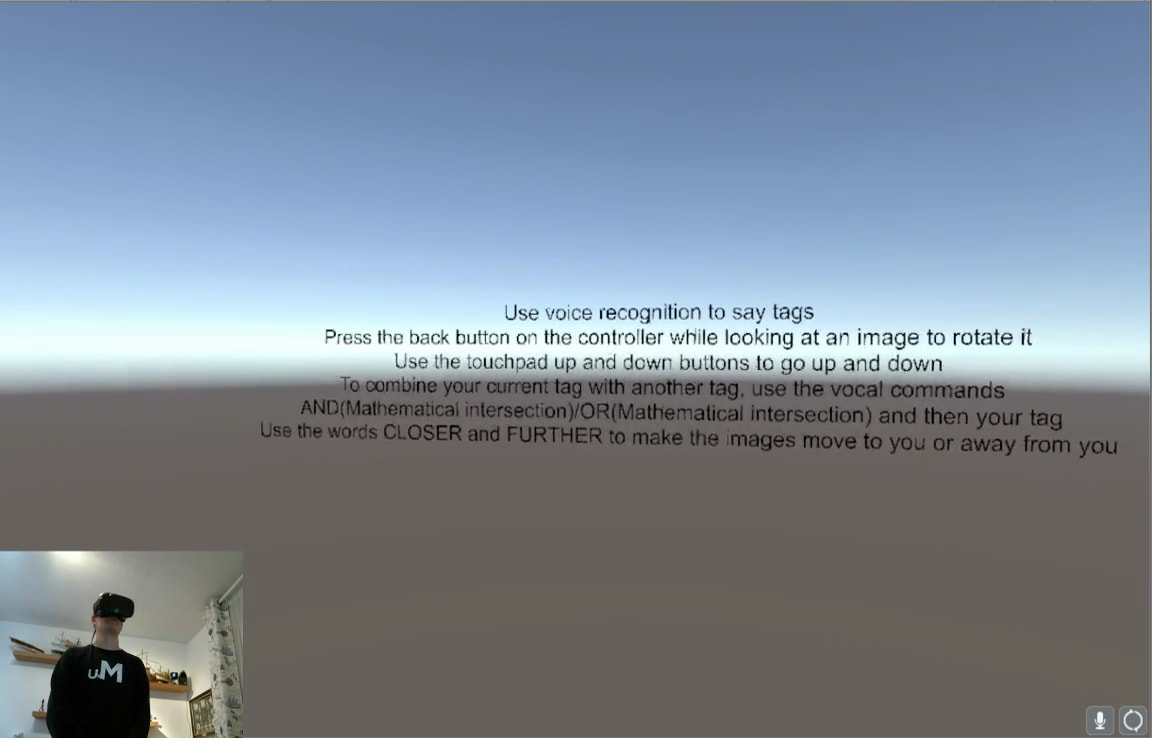
\includegraphics[width=\textwidth]{img/Help.jpg}
\end{figure}

\begin{figure}[h]
  \label{fig:cntr}
  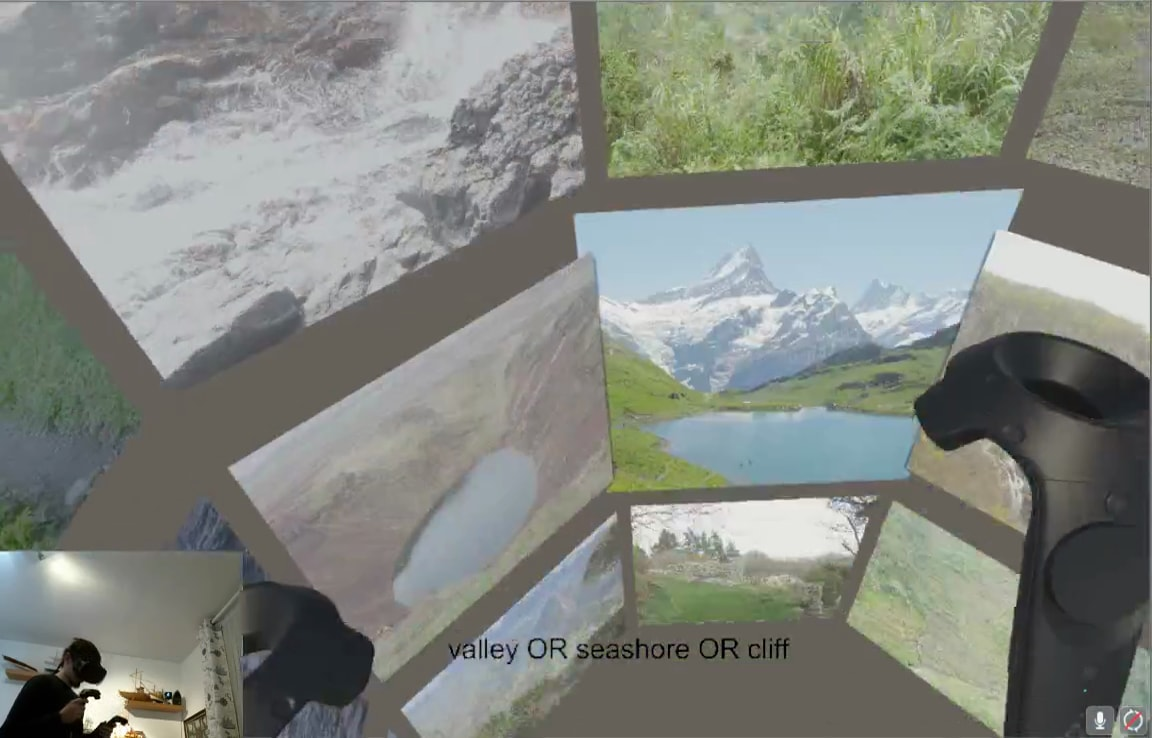
\includegraphics[width=\textwidth]{img/Controllers.jpg}
\end{figure}

\begin{figure}[h]
  \label{fig:1tag}
  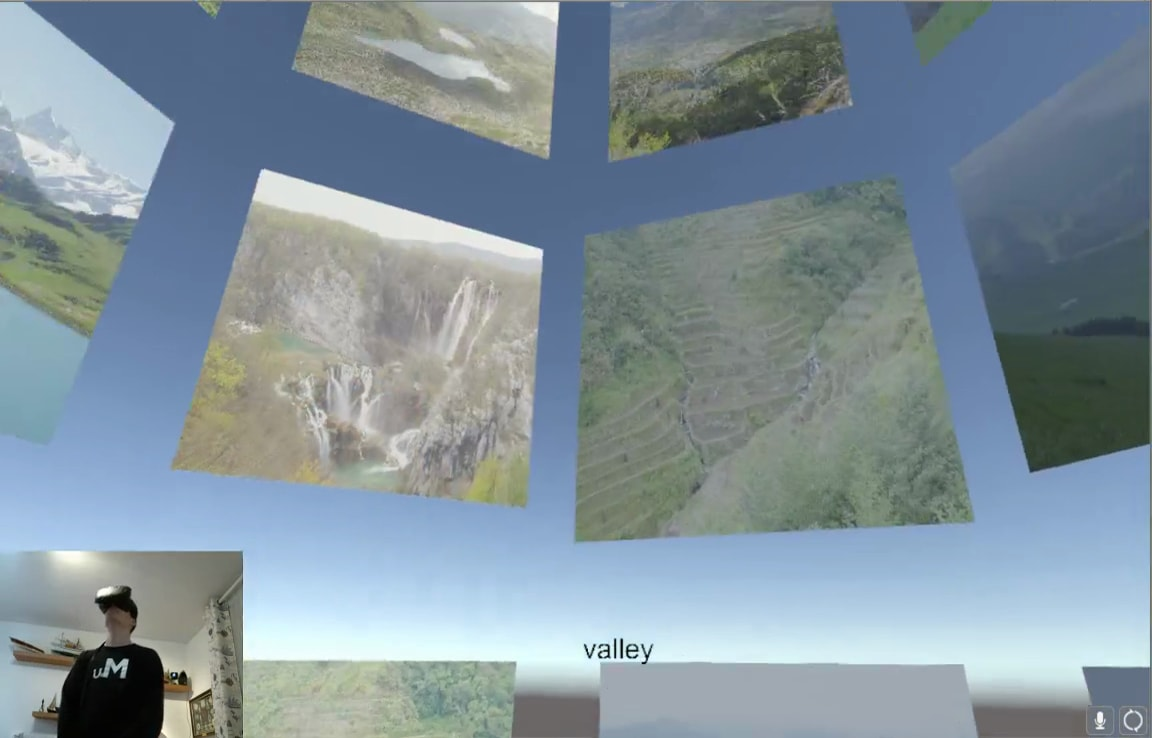
\includegraphics[width=\textwidth]{img/SimpleTag.jpg}
\end{figure}

\begin{figure}[h]
  \label{fig:3tag}
  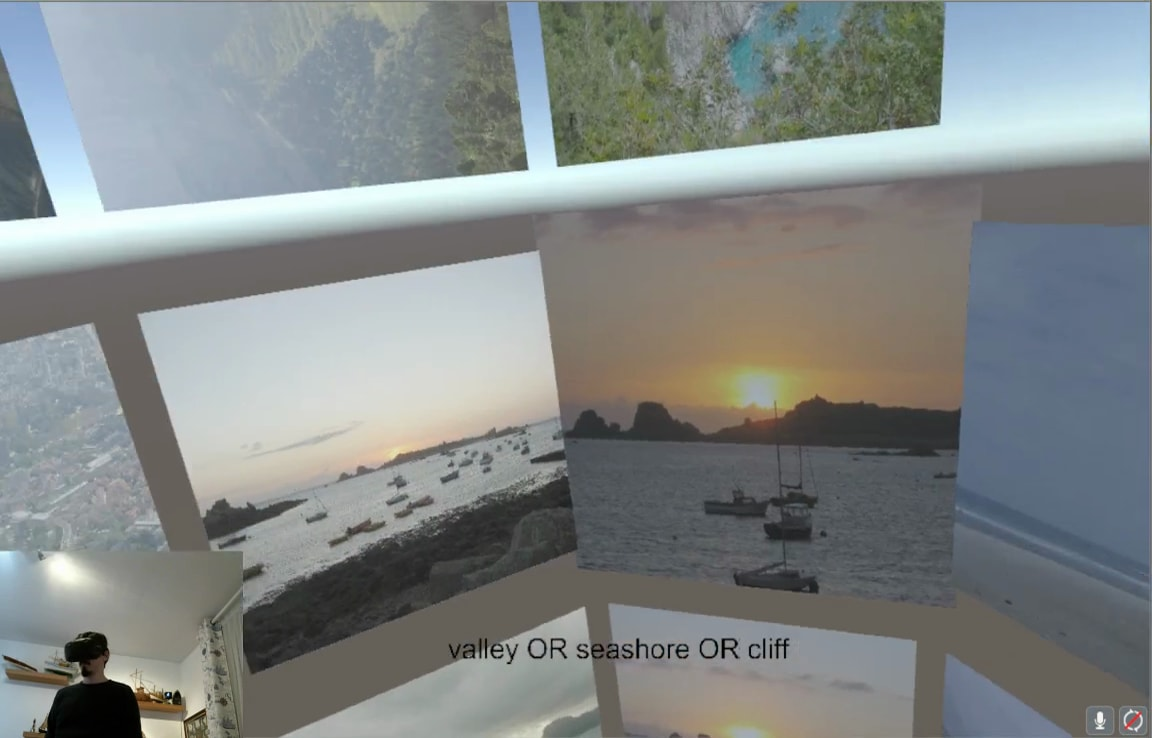
\includegraphics[width=\textwidth]{img/TripleTag.jpg}
\end{figure}

\begin{figure}[h]
  \label{fig:suggestions}
  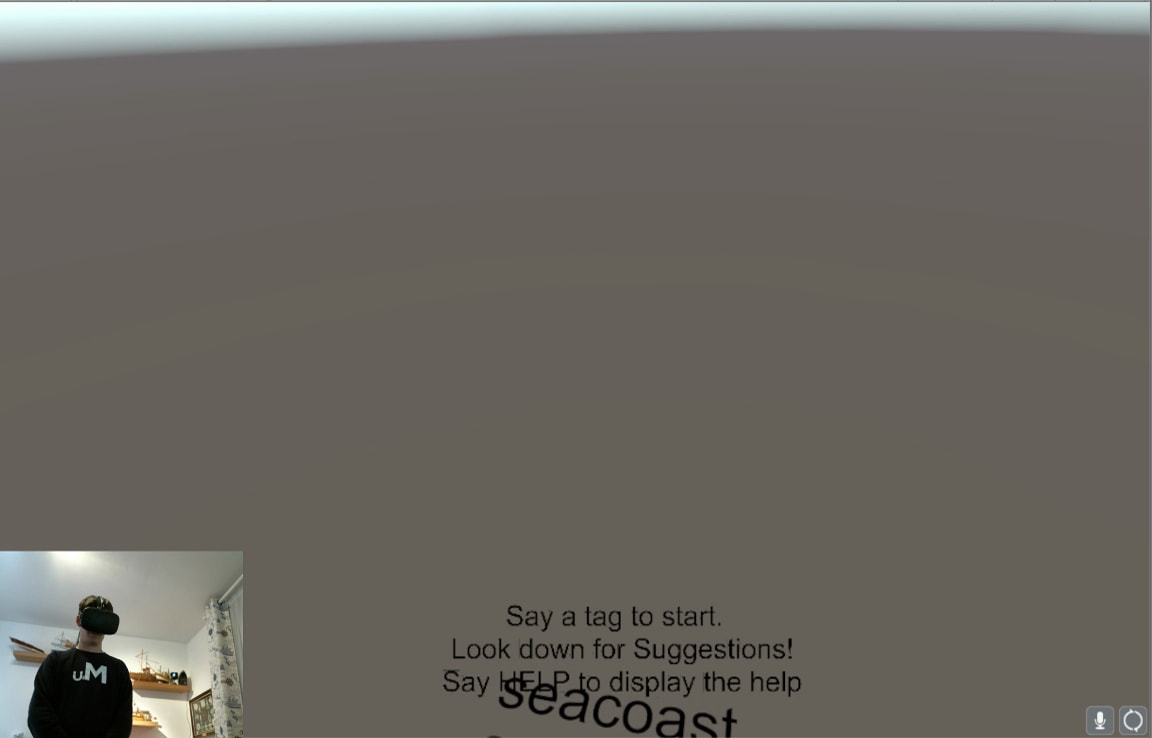
\includegraphics[width=\textwidth]{img/Start.jpg}
\end{figure}

\begin{figure}[h]
  \label{fig:vive}
  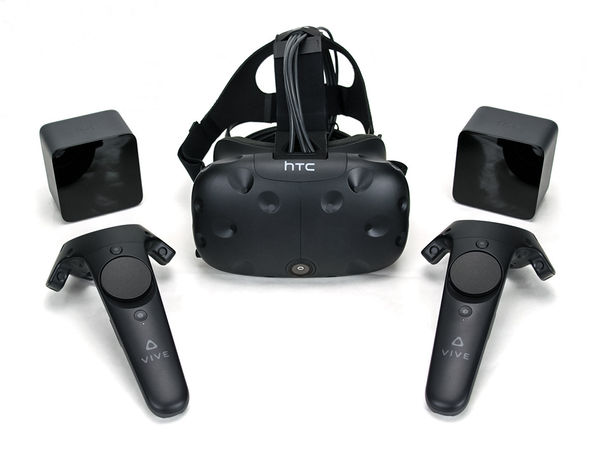
\includegraphics[width=\textwidth]{img/vive.jpg}
\end{figure}

\end{document}


\end{document}




